\documentclass[9pt]{beamer}
\usetheme{CambridgeUS}
\usepackage{graphicx}

\title{\textbf{TimeTraveler: The Lost Key}}
\author{ \textbf{Varshini}, \textbf{Akshaya}, \textbf{Chandana}, \textbf{Mani Harshitha}, \textbf{Yaaghnetha}}

\begin{document}

\begin{frame}
\titlepage
\end{frame}

\begin{frame}
    \frametitle{PROJECT DESCRIPTION}
    \begin{itemize}
        \item A time travel adventure game where the player must find a lost key to return to the present.
        \item The player’s time machine malfunctions, causing them to land in an unknown timeline.
        \item The player must navigate through various historical or futuristic settings to find the key.
        \item After completing certain levels and get the key, the player will return to the present and completes the game.
    \end{itemize}
\end{frame}


\begin{frame}
    \frametitle{FEATURES}
    \begin{itemize}
        \item \textbf{Player Movement}: Navigation of Character and Camera through arrow keys, Collision Detection and Rotation.
        \item \textbf{3D Environment}: Maze generation using Recursive Backtracking Algorithm and converion of 2D map to 3D. 
        \item \textbf{3D Environment}: Use of realistic wall and floor textures and skybox integration
        \item \textbf{Minimap}: The minimap updates in real-time to reflect the player’s current position within the maze.
        \item \textbf{Minimap}: The minimap has an end-marker, and reflects the maze's layout accurately.
        \item \textbf{Camera}: The third-person camera provides an follow up to the character making the user to easily control the character.
        \item \textbf{Audio Integration}: Sound effects are triggered when the player collides with walls or reaches the end of the maze.
        \item \textbf{User Interface}: Addition of loading screen and responsive design makes it easy for different device widths.
    \end{itemize}
\end{frame}



\begin{frame}
\frametitle{Tech Stack}
\begin{itemize}
    \item \textbf{Frontend}: Three.js, WebGL, HTML Canvas
    \item \textbf{3D Character Modelling and Designs}: Blender, Clara.io, SketchFab, Playground
    \item \textbf{Sound}: Three.js Audio API
\end{itemize}
\end{frame}



\begin{frame}
    \frametitle{CHALLENGES FACED}
    \begin{itemize}
        \item \textbf{Collision Detection}: Used bounding boxes(THREE.Box3), optimized collision checks.
        \item \textbf{Character loading}: Had issues with rendering the scene before models/textures fully load.
        \item \textbf{Minimap generation}: Integrating 2D elements like minimaps with the 3D scene was more challenging than rendering 3D scene.
        \item \textbf{3D Map implementation}: Mapping 2D maze to 3D walls.
        \item \textbf{Sound Effects and Character handling}: Adding sounds and modelling the character.
        \item \textbf{Project Management}: Managing timeline of all the team members.
        \item \textbf{Error Handling and Debugging}: Used try-catch blocks, logged errors, debugged with browser tools.
    \end{itemize}
\end{frame}


\begin{frame}
    \frametitle{Development Progress}
    \begin{itemize}
        \item \textbf{Project Planning: June 28-July 05}: 
        \begin{itemize}
            \item Conceptualized the game idea and set project goals.
            \item Established the timeline whom have to work for which part of the project.
        \end{itemize}
        \vspace{0.5em}
        
        \item \textbf{Design Phase: July 09-July 13}: 
        \begin{itemize}
            \item Designed the 3D maze layout, homepage and selected textures.
            \item Planned the user interface, including the minimap.
        \end{itemize}
        \vspace{0.5em}
        
        \item \textbf{Implementation: July 13-Aug 10}: 
        \begin{itemize}
            \item Set up the Three.js scene and added lighting.
            \item Implemented player movement, collision detection, and minimap integration.
        \end{itemize}
        \vspace{0.5em}
        
        \item \textbf{Optimization: Aug 10-Aug 12}: 
        \begin{itemize}
            \item Minimap Integration, Character Loading.
            \item Improved collision detection for better performance.
        \end{itemize}
        
        \vspace{0.5em}
        \item \textbf{Testing and Debugging: Aug 13-Aug 16}: 
        \begin{itemize}
            \item Testing and fixed bugs.
            \item Ensured responsive User Interface.
        \end{itemize}
    \end{itemize}
\end{frame}
        
\begin{frame}
    \begin{itemize}
        \item \textbf{Final Adjustments}: 
        \begin{itemize}
            \item Polished visuals and refined gameplay mechanics and character controls.
        \end{itemize}
        \vspace{0.5em}

        \item \textbf{Documentation}: 
        \begin{itemize}
            \item Documented code and created user guides.
            \item Compiled a project report summarizing the development process.
        \end{itemize}
        
        \vspace{0.5em}

        \item \textbf{Tools and Technologies}: 
        \begin{itemize}
            \item Utilized \textbf{Three.js, WebGL}, and \textbf{JavaScript} for development.
            \item Used \textbf{Clara.io, Blender, SketchFab, Adobe Firefly, Playground} for Character design and modelling, Key, Environment.
            \item Managed version control and collaboration using \textbf{Git}.
        \end{itemize}
    \end{itemize}
\end{frame}



\begin{frame}
    \frametitle{OUTCOMES}
    \begin{figure}[h]
        \centering
        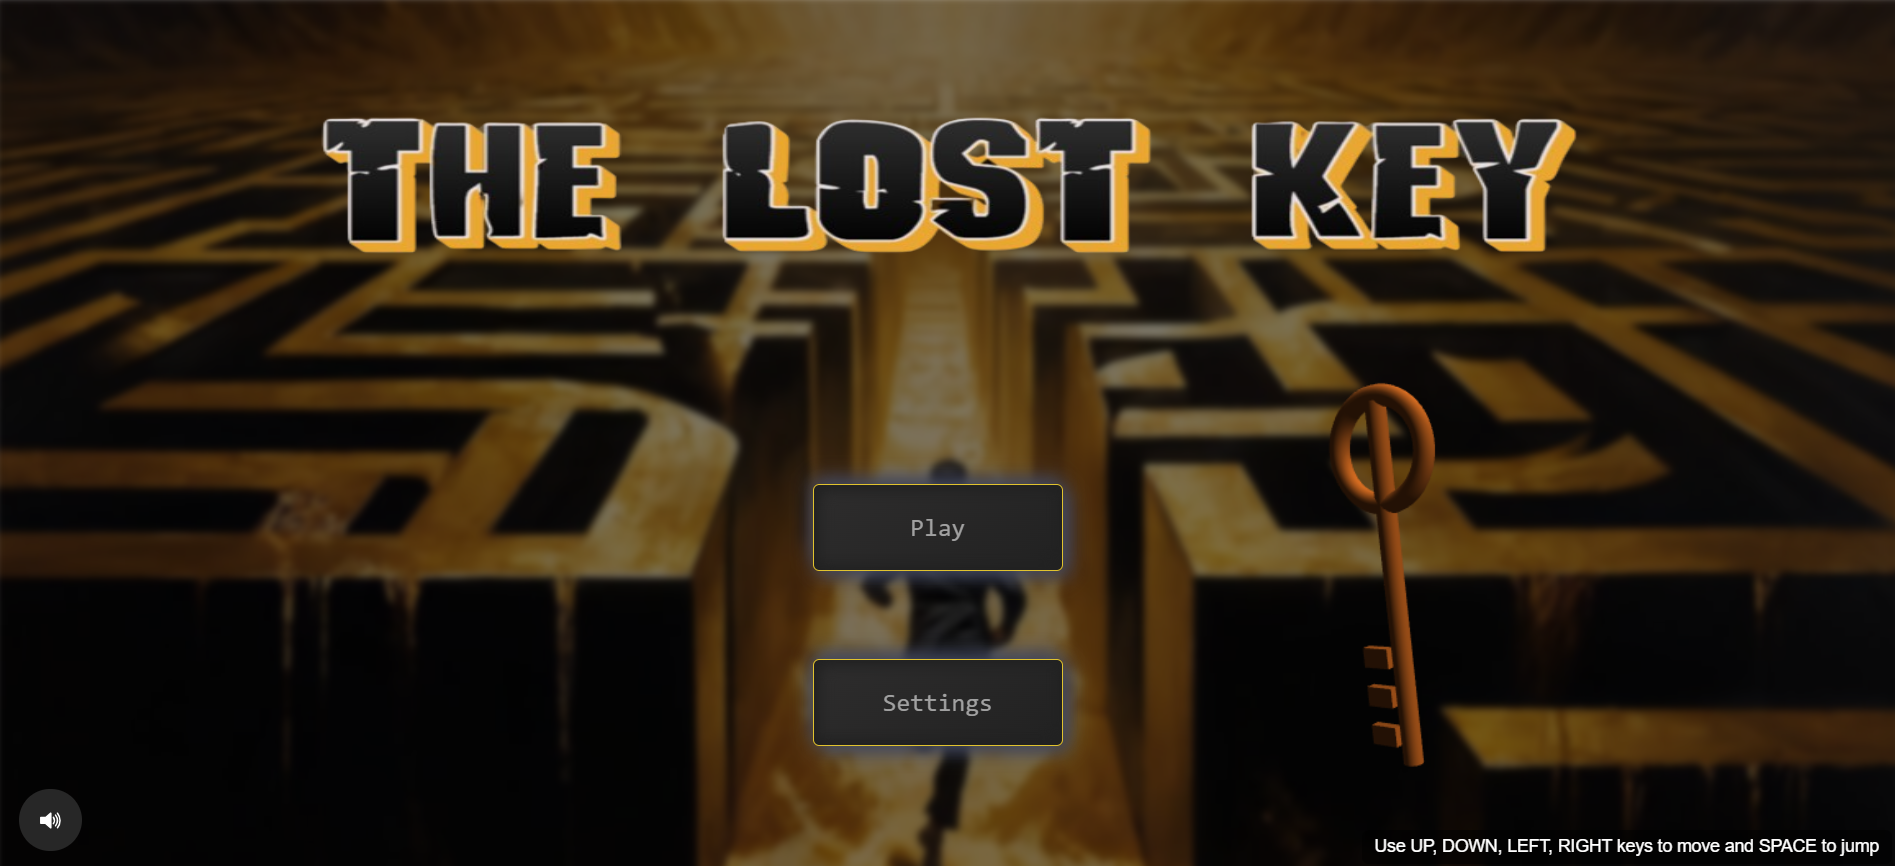
\includegraphics[width=0.9\textwidth, height=0.8\textheight]{HomePage.png}
        \caption{HomePage}
    \end{figure}
\end{frame}


\begin{frame}
    \frametitle{OUTCOMES}
    \begin{figure}[h]
        \centering
        \includegraphics[width=0.9\textwidth, height=0.8\textheight]{level1.png}
        \caption{LEVEL 1}
    \end{figure}
\end{frame}

\begin{frame}
    \frametitle{OUTCOMES}
    \begin{figure}[h]
        \centering
        \includegraphics[width=0.9\textwidth, height=0.8\textheight]{level2.png}
        \caption{LEVEL 2}
    \end{figure}
\end{frame}

\begin{frame}
    \frametitle{OUTCOMES}
    \begin{figure}[h]
        \centering
        \includegraphics[width=0.9\textwidth, height=0.8\textheight]{level3.png}
        \caption{LEVEL 3}
    \end{figure}
\end{frame}

\begin{frame}
    \frametitle{OUTCOMES}
    \begin{figure}[h]
        \centering
        \includegraphics[width=0.9\textwidth, height=0.7\textheight]{maze.png}
        \caption{MAZE}
    \end{figure}
\end{frame}


\begin{frame}
    \frametitle{INSPIRATIONS}
    \begin{itemize}
        \item https://summer-afternoon.vlucendo.com/
        \item https://github.com/demonixis/Maze3D
    \end{itemize}
\end{frame}


\begin{frame}
    \frametitle{LESSONS AND SKILLS LEARNED}
    \begin{itemize}
        \item \textbf{Technical Skills}:
        \begin{itemize}
            \item Learnt a lot in Three.js, WebGL, and JavaScript for 3D game development.
            \item Improved understanding of 3D graphics, including lighting, shading, and camera controls.
            \item Debugging complex issues, such as collision detection and asynchronous loading.
        \end{itemize}
        \vspace{0.5em}
        
        \item \textbf{Collaboration and Communication}:
        \begin{itemize}
            \item Enhanced collaboration skills through version control and teamwork.
            \item Improved communication by documenting the project and presenting it effectively.
        \end{itemize}
        \vspace{0.5em}
        
        \item \textbf{Adaptability}:
        \begin{itemize}
            \item Developed the ability to quickly learn and adapt to new tools and technologies, here a completely new library.
            \item Improved flexibility in problem-solving by trying different approaches to achieve planned results.
        \end{itemize}
        \vspace{0.5em}

        \item \textbf{Future Improvements}:
        \begin{itemize}
            \item Multiplayer options and leaderboard integration integrating backend.
            \item Addition of more number of levels with different environments.
        \end{itemize}
    \end{itemize}
    \end{frame}
    

\begin{frame}
    \frametitle{CONTRIBUTION TO THE PROJECT}
    \begin{itemize}
        \item \textbf{HomePage}: Akshaya - Complete
            \begin{itemize}
                \item Included Play, Quit, Sound buttons, and Instructions. 3D Key Integration and Linking of HomePage to Level 1.
            \end{itemize}
        \vspace{0.5em}
        \item \textbf{Level 1}: Chandana, Varshini
            \begin{itemize}
                \item Description: The player is stuck in a cave, where he has to reach the end point with the help of minimap.
                \item Path Generation: Random path generation.
                \item Chandana: Sound, Player Movements, Collision Detection.
                \item Varshini: Maze and Minimp Generation, Setting up of scene and environment, End Point Detection, Linking of level 1 to 2 and player loading.
            \end{itemize}
            \vspace{0.5em}
        \item \textbf{Level 2}: Yaaghnetha - Complete
            \begin{itemize}
                \item Description: The player is stuck in an ancient maze and has to reach the end point from his current position with the help of minimap.
                \item Maze Generation: Generated 2D maze and integrated the maze data to make a 3D model of it.
                \item Setting up of scene which includes, minimap, camera, floor and wall textures, skybox integration and player loading, Linking of level 2 to 3.
                \item Inclusion of physics: Collsion Detection, Player Movements, End Point Detection.
            \end{itemize}
        \end{itemize}
\end{frame}

\begin{frame}
    \begin{itemize}
        \item \textbf{Level 3}: Varshini - Complete
            \begin{itemize}
                \item Description: The player is now stuck in a futuristic era and has to jump through the buildings and get the final key to complete the game(no help of minimap).
                \item Setting up of scene which includes, camera, floor and building textures, and player loading, Linking of level 3 to HomePage.
                \item Inclusion of physics: Collsion Detection, Player Movements, End Point Detection.
            \end{itemize}
            \vspace{0.5em}
        \item \textbf{Character}: Mani Harshitha
            \begin{itemize}
                \item Designed the game character from scratch using Blender.
            \end{itemize}
            \vspace{0.5em}
        \item \textbf{Sound}: Chandana
            \begin{itemize}
                \item Integrated sound during collision detection for all the three levels.
            \end{itemize}
    \end{itemize}
\end{frame}
    

\begin{frame}
\centering
\Huge
\emph{THANK YOU}
\end{frame}

\end{document}
